% !TEX TS-program = pdflatex
% !TEX encoding = UTF-8 Unicode

% This is a simple template for a LaTeX document using the "article" class.
% See "book", "report", "letter" for other types of document.

\documentclass[11pt]{article} % use larger type; default would be 10pt

\usepackage[utf8]{inputenc} % set input encoding (not needed with XeLaTeX)

%%% Examples of Article customizations
% These packages are optional, depending whether you want the features they provide.
% See the LaTeX Companion or other references for full information.

%%% PAGE DIMENSIONS
\usepackage{geometry} % to change the page dimensions
\geometry{a4paper} % or letterpaper (US) or a5paper or....
% \geometry{margin=2in} % for example, change the margins to 2 inches all round
% \geometry{landscape} % set up the page for landscape
%   read geometry.pdf for detailed page layout information

\usepackage{graphicx} % support the \includegraphics command and options

% \usepackage[parfill]{parskip} % Activate to begin paragraphs with an empty line rather than an indent

%%% PACKAGES
\usepackage[font=small,format=plain,labelfont=bf,up,textfont=it,up]{caption} % for nice captions
\usepackage{booktabs} % for much better looking tables
\usepackage{array} % for better arrays (eg matrices) in maths
\usepackage{paralist} % very flexible & customisable lists (eg. enumerate/itemize, etc.)
\usepackage{verbatim} % adds environment for commenting out blocks of text & for better verbatim
\usepackage{subfig} % make it possible to include more than one captioned figure/table in a single float
% These packages are all incorporated in the memoir class to one degree or another...
\usepackage[table]{xcolor} % colors for the tables


%%% HEADERS & FOOTERS
\usepackage{fancyhdr} % This should be set AFTER setting up the page geometry
\pagestyle{fancy} % options: empty , plain , fancy
\renewcommand{\headrulewidth}{0pt} % customise the layout...
\lhead{}\chead{}\rhead{}
\lfoot{}\cfoot{\thepage}\rfoot{}

%%% SECTION TITLE APPEARANCE
\usepackage{sectsty}
\allsectionsfont{\sffamily\mdseries\upshape} % (See the fntguide.pdf for font help)
% (This matches ConTeXt defaults)

%%% ToC (table of contents) APPEARANCE
\usepackage[nottoc,notlof,notlot]{tocbibind} % Put the bibliography in the ToC
\usepackage[titles,subfigure]{tocloft} % Alter the style of the Table of Contents
\renewcommand{\cftsecfont}{\rmfamily\mdseries\upshape}
\renewcommand{\cftsecpagefont}{\rmfamily\mdseries\upshape} % No bold!

%%% BIBLIOGRAPHY
\usepackage{natbib}
\usepackage{url}

\usepackage{subfig}


%%% END Article customizations

%%% The "real" document content comes below...

\title{Automated Reasoning in AI\\
Assignment 3: Description Logic}
\author{Armon Toubman \and Torec Luik}
%\date{} % Activate to display a given date or no date (if empty),
         % otherwise the current date is printed

\begin{document}
\maketitle

\section{Tableau algorithm}
\label{sec:tableau}

We use the following mapping from Description Logic to LoTREC. It is similar to the example given in the assignment except for some of the LoTREC displays.

\begin{table}[h]
\begin{center}
\begin{tabular}{l c c c c c c}
$\mathcal{ALC}$ syntax & $\neg C$ & $C \sqcap D$ & $C \sqcup D$ & $\exists r.C$ & $\forall r.C$ & $\top \equiv D$\\
LoTREC connective & \texttt{not} $C$ & \texttt{and} $C D$ & \texttt{or} $C D$ & \texttt{some} $r$ $C$ & \texttt{only} $r$ $C$ & \texttt{tbox} $D$\\
LoTREC display & $\sim$ $C$ & $C$ $^\wedge$ $D$ & $C$ v $D$ & $r$ some $C$ & $r$ only $C$ & $\top$ = $D$\\
\end{tabular}
\end{center}
\end{table}

To indicate $\top$ and $\bot$ we use two connectors \texttt{true} and \texttt{false}, both with arity 1. The actual variable used with these connectors is disregarded. The representation of lists of formulas and of problem instances are again much like the example:

\begin{table}[h]
\begin{center}
\begin{tabular}{l c c}
LoTREC connective & \texttt{add} $\phi$ $\psi$ & \texttt{input} $\mathcal{T}$ $C$\\
LoTREC display & $\phi$ \& $\psi$ & INPUT: TBox = $\mathcal{T}$; ABox = $C$\\
\end{tabular}
\end{center}
\end{table}

Because the only differences in our encoding and the example encoding in the assignment are in the LoTREC display, the LoTREC input of formulas is done in the same way as the example formula used in Figure 1 and 2 of the assignment:

\begin{table}[h]
\begin{center}
\begin{tabular}{c}
(\{$\top \equiv \exists s.C$, $\top \equiv \forall r.(\neg C \sqcup D)$\}, $\exists r.(C \sqcap D)$)\\
\texttt{input add tbox some S C tbox only R or not C D some R and C D}\\
\end{tabular}
\end{center}
\end{table}

All connectors, rules, strategies and example formulas can of course be found in our LoTREC file.

\textcolor{red}{Waarom firstRule, waarom allRules rond block/some/tbox}

\section{Reasoning problems}
\label{sec:reasoning}

Solve the following decision problems supporting yourself with your implemen-
tation of tableau algorithm.

\subsection{}

\begin{center}
Is $\exists r.D$ satisfiable with regard to $\mathcal{T}$ = \{ $\top \equiv \exists s.C$, $\top \equiv \forall r.(\bot \sqcup E)$ \}?
\end{center}

\begin{enumerate}
\item State the problem.
\item Reduce the problem to the corresponding concept satisfiability problem (as shown during the lecture).
\item Apply the necessary syntactic transformations to the TBox and the concept so that the conditions, listed in the previous task, are satisfied.
\item Translate the result into the input formula for your tableau implementation. Please, type and save this formula also in your implementation file *.xml [LoTREC tab: Predefined Formulas]
\item Use your implementation of the tableau to compute a tableau tree for this formula.
\item State the result of the computation (is the tableau closed or open?) If the tableau is open include a picture of one of its open branches in the report [LoTREC menu: Premodels/Export Premodel...].
\item Based on the result of the computation provide the answers to the following problems: 1) the original decision problem; 2) the corresponding concept satisfiability problem that you solved with the tableau algorithm.
\end{enumerate}

\subsection{}

\begin{center}
Is $D \sqcap E$ subsumed by $\exists r.B$ in $\mathcal{T}$ = \{ $C \sqsubseteq \neg A$, $D \sqsubseteq \forall r.(A \sqcup B)$, $E \sqsubseteq \exists r.C$\}?
\end{center}

\begin{enumerate}
\item State the problem.
\item Reduce the problem to the corresponding concept satisfiability problem (as shown during the lecture).
\item Apply the necessary syntactic transformations to the TBox and the concept so that the conditions, listed in the previous task, are satisfied.
\item Translate the result into the input formula for your tableau implementation. Please, type and save this formula also in your implementation file *.xml [LoTREC tab: Predefined Formulas]
\item Use your implementation of the tableau to compute a tableau tree for this formula.
\item State the result of the computation (is the tableau closed or open?) If the tableau is open include a picture of one of its open branches in the report [LoTREC menu: Premodels/Export Premodel...].
\item Based on the result of the computation provide the answers to the following problems: 1) the original decision problem; 2) the corresponding concept satisfiability problem that you solved with the tableau algorithm.
\end{enumerate}

\subsection{}

\begin{center}
Is the ABox \{$C(a)$\} consistent with regard to $\mathcal{T}$ = \{$\top \equiv \forall r.B \sqcap \forall s.C$, $\top \equiv \neg \forall r.(\neg C \sqcap B)$, $\top \equiv \exists s.\top$\}?
\end{center}

\begin{enumerate}
\item State the problem.
\item Reduce the problem to the corresponding concept satisfiability problem (as shown during the lecture).
\item Apply the necessary syntactic transformations to the TBox and the concept so that the conditions, listed in the previous task, are satisfied.
\item Translate the result into the input formula for your tableau implementation. Please, type and save this formula also in your implementation file *.xml [LoTREC tab: Predefined Formulas]
\item Use your implementation of the tableau to compute a tableau tree for this formula.
\item State the result of the computation (is the tableau closed or open?) If the tableau is open include a picture of one of its open branches in the report [LoTREC menu: Premodels/Export Premodel...].
\item Based on the result of the computation provide the answers to the following problems: 1) the original decision problem; 2) the corresponding concept satisfiability problem that you solved with the tableau algorithm.
\end{enumerate}

\section{Strategies}
\label{sec:strategies}

\subsection{Blocking}

The blocking rule should only be applied when no other rules are applicable on the branch to guarantee termination and completeness of the algorithm. We can show that this is the case using our \texttt{WrongBlocking} strategy. This strategy has the blocking rule at the beginning of the strategy instead of at the end. Also, compared to our default strategy \texttt{Strategy}, the blocking rule, some rule and tbox rule are no longer in an \texttt{allRules} block. To show the difference we use this formula (in the LoTREC file under Predefined formulas, Wrong Blocking):

\begin{center}
\texttt{input tbox some R or U V some R V}
\end{center}

If we process this formula with the default strategy, which we assume to be complete and sound, we get a forest with 36 premodel trees. However, if we process the same formula with the wrongly blocking strategy, we get only 16 premodel trees. This strategy is obviously not exploring some premodels that the default strategy is. In other words, the wrongly blocking strategy does not guarantee completeness.

\subsection{Ordering}

We have to fit nine rules into our strategy: TruthRule, FalsumRule, OnlyRule, AndRule, OrRule, Clash, Block, SomeRule and TBoxRule. The TruthRule might not be necessary in our current setup, but the others all need a place. 

It is most efficient to use a repeated firstRule strategy with Clash as the first rule, because this will allow the algorithm to find a clash as fast as possible and to stop working on that branch. Consider the following strategy: 

\begin{center}
\texttt{add add add A not A and B or C D some X or A B}
\end{center} 

Here we are given the formulae "A", "$\neg A$", "$B\sqcap (C \sqcup D)$" and "$\exists X. A \sqcup B$". If Clash is not applied before the AndRule, OrRule and SomeRule, the latter formulae will be looked into first, while we are already given a contradiction. Always applying Clash first can only save space and time. Since FalsumRule is similar to Clash (except we look for a Bottom sign instead of a contradiction), this rule should be applied soon after Clash. Using the firstRule strategy, we make sure these are checked at every possible opportunity.
If the TruthRule is used, it should be applied next because if it is applicable, it will also stop the algorithm after combining it with the FalsumRule.

At the other end of the strategy, we should find the SomeRule (and its companion rules Block and TBoxRule). The SomeRule has no interaction with the rest of the formulae in the current node and a succesful application will only increase the size of the solution tree. For this reason, it seems beneficial to the size and completion time of the algorithm to first apply all rules that can be applied before using the SomeRule, in the hope of finding a Clash first. The effect of misusing the SomeRule can be found by applying the WrongBlocking strategy to the efficiency-testing formula.

Now we are left with the OnlyRule, the AndRule and the OrRule. From these, the OrRule uses the greatest amount of space by copying the whole tree. As such, it should be applied last of these three, once again in the hopes of finding a Clash earlier. Between the OnlyRule and the AndRule there does not seem to be a lot of difference, seeing as both might produce a contradiction with one application. However, the AndRule will try to fill two lines while the OnlyRule fills only one line.

Thereby, we reason that the most efficient ordering of rules is the following:

\begin{enumerate}
\item Clash
\item FalsumRule
\item TruthRule
\item OnlyRule
\item AndRule
\item OrRule
\item Block, SomeRule and TBoxRule
\end{enumerate}

\section{Extensions}
\label{sec:extensions}

We have implemented the Transitive roles and Role hierarchies extensions.

\subsection{Transitive roles}

To implement transitive roles, we added a new operator and a new rule. The operator:

\begin{table}[h]
\begin{center}
\begin{tabular}{l c}
LoTREC connective & \texttt{trans} $C$ \\
LoTREC display & $+C$ \\
\end{tabular}
\end{center}
\end{table}

This unary operator indicates that the argument role is transitive. We have implemented it in such a way that a transitivity statement is given as a seperate statement for the TBox or ABox. We have added a rule \texttt{TransitiveRoleSome} that takes such a transitivity statement and nested \texttt{some} statements that it can process:

\begin{table}[h]
\begin{center}
\begin{tabular}{l l}
\texttt{TransitiveRoleSome} & \\
\hline
Conditions: & \texttt{hasElement node trans \_t} \\
 & \texttt{hasElement node some \_t some \_t some \_b} \\
Actions: & \texttt{add node some \_t \_b} \\
\hline
\end{tabular}
\end{center}
\end{table}

The application of transitivity can be shown with the example formula from the assignment:

\begin{table}[h]
\begin{center}
\begin{tabular}{l l}
TBox & $\exists{}hasPart.(\exists{}hasPart.(\exists{}hasPart.Component))$ \\
ABox & $\exists{}hasPart.Component$ \\
\\
LoTREC input & \texttt{input add tbox trans HasPart} \\
 & \texttt{tbox some HasPart some HasPart some HasPart Component}\\
 & \texttt{some HasPart Component} \\
\end{tabular}
\end{center}
\end{table}

The effect is most noticable in the first node of our premodels as shown in Figure~\ref{fig:transitivity}. The transitivity rule breaks down "HasPart some (HasPart some (HasPart some Component))" to "HasPart some (HasPart some Component)" and "HasPart some Component", although the latter is already given by the ABox.

\begin{figure}[h]
\begin{center}
\subfloat{
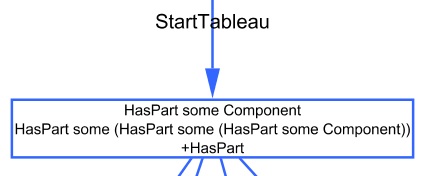
\includegraphics[scale=0.5]{premodelzondertransitivity}
}
\subfloat{
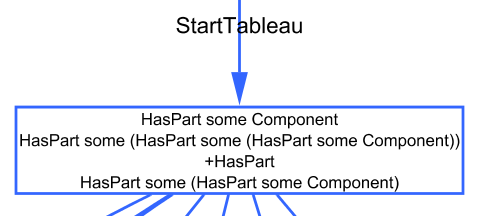
\includegraphics[scale=0.4]{premodelmettransitivity}
}
\caption{On the left, the first node in the premodel without transitivity, using strategy \texttt{Strategy}. On the right, the first node in the premodel without transitivity, using strategy \texttt{Strategy}.}
\label{fig:transitivity}
\end{center}
\end{figure}

\subsection{Role hierarchies}

To implement role hierarchies, we added a new operator and a new rule. The operator:

\begin{table}[h]
\begin{center}
\begin{tabular}{l c}
LoTREC connective & \texttt{subrole} $C D$ \\
LoTREC display & $C subrole of D$ \\
\end{tabular}
\end{center}
\end{table}

The application of role hierarchies can be shown with the example formula from the assignment:

\begin{table}[h]
\begin{center}
\begin{tabular}{l l}
TBox & $\exists{}Painted.Painting$ \\
ABox & $\forall{}Created.\neg{}Painting$ \& $Painted\sqsubseteq{}Created$ \\
\\
LoTREC input & \texttt{input tbox some Painted Painting} \\
 & \texttt{add only Created not Painting}\\
 & \texttt{subrole Painted Created} \\
\end{tabular}
\end{center}
\end{table}

For this formula, the strategy with subroles creates a different premodel than the strategy without subroles. The premodel with subroles creates a clash while the premodel without subroles doesnt. The premodels are shown in Figure \ref{fig:zondersubrole} and \ref{fig:metsubrole}.



\begin{figure}
\begin{center}
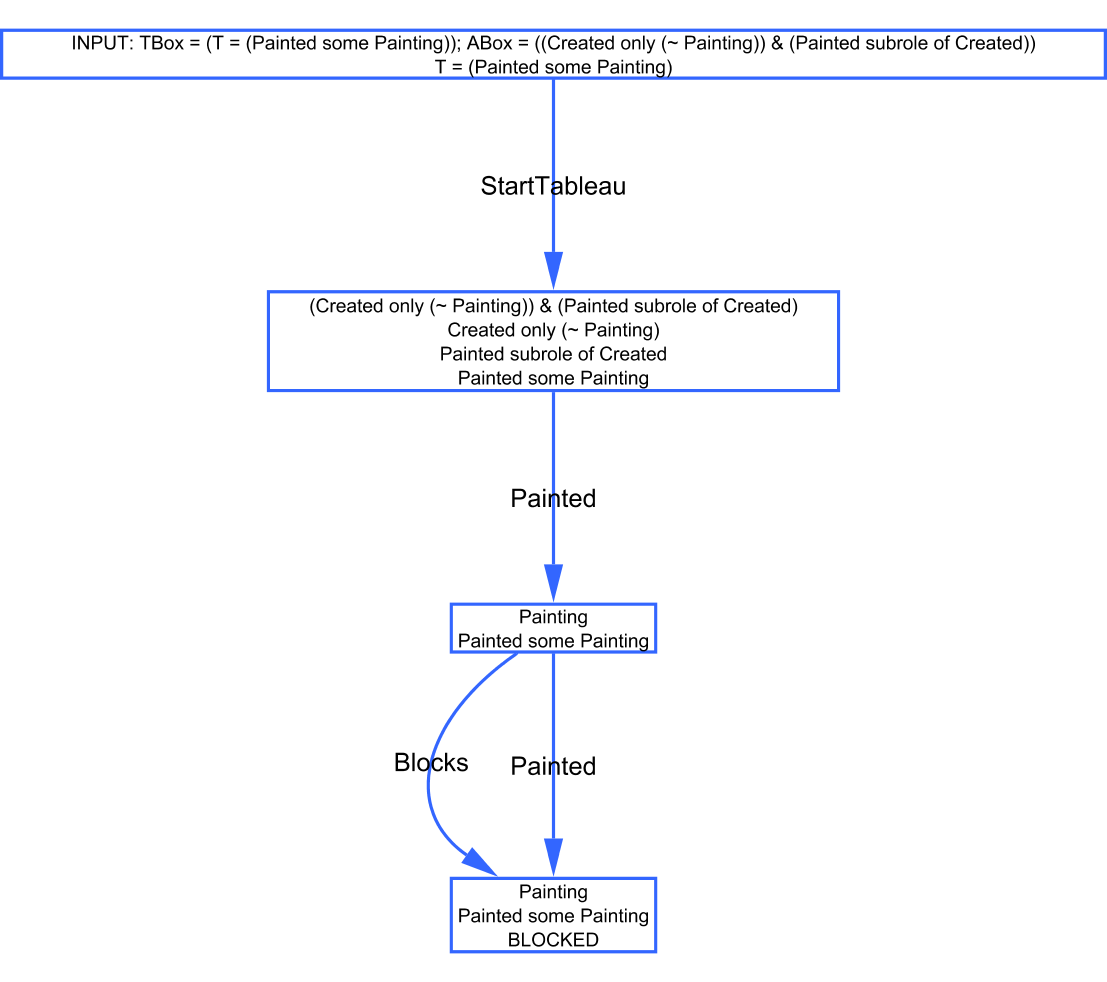
\includegraphics[scale=0.4]{premodelzondersubrole}
\caption{Premodel of the example formula for Role hierarchies. This premodel was created with the default strategy \texttt{Strategy}. The concept is satisfiable.}
\label{fig:zondersubrole}
\end{center}
\end{figure}

\begin{figure}
\begin{center}
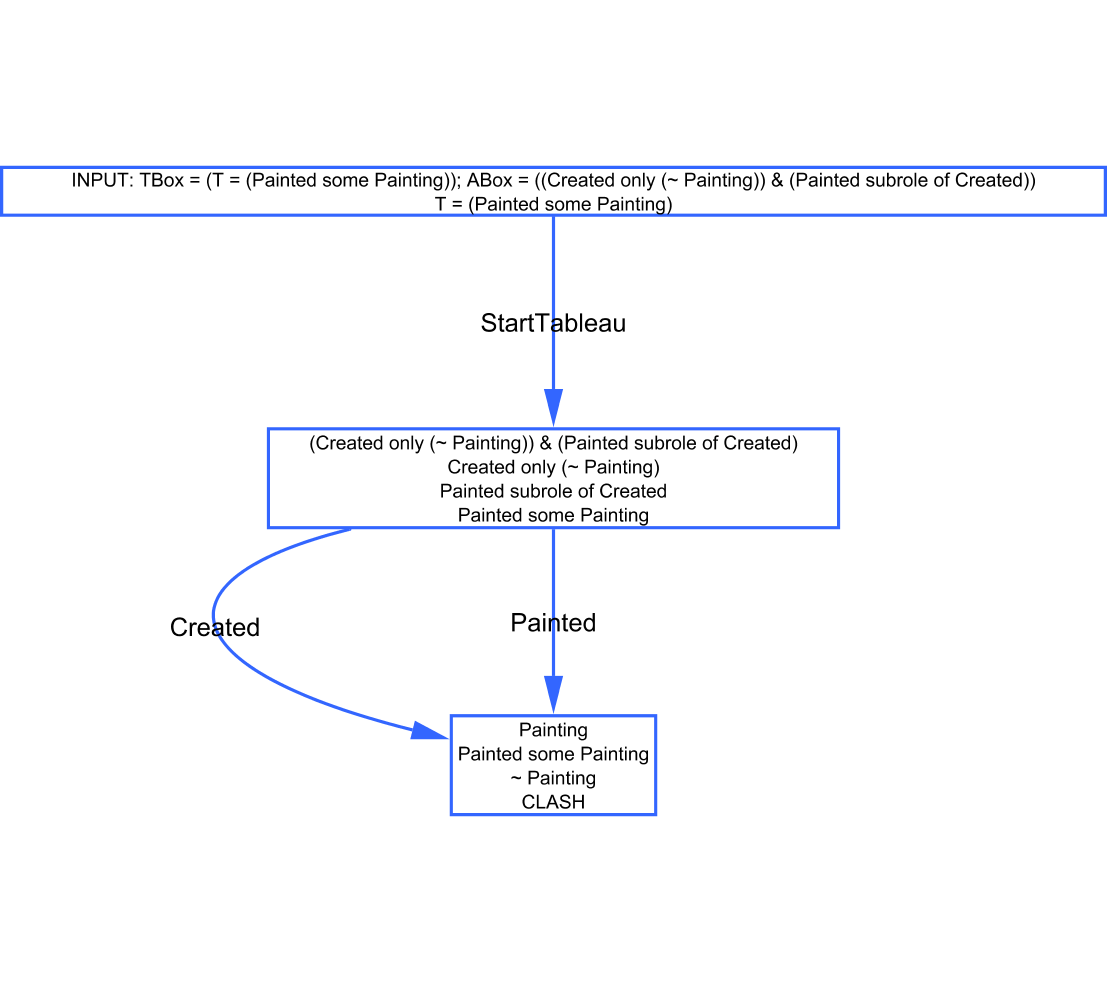
\includegraphics[scale=0.4]{premodelmetsubrole}
\caption{Premodel of the example formula for Role hierarchies. This premodel was created with the extended strategy \texttt{StrategyWithRoleHierarchies}. The concept is unsatisfiable.}
\label{fig:metsubrole}
\end{center}
\end{figure}



\textcolor{red}{$\rightarrow$ references? wat? $\leftarrow$}

\bibliographystyle{plainnat}
\bibliography{ref}

\end{document}
